\documentclass[10pt,twocolumn,letterpaper]{article}

\usepackage{iccv}
\usepackage{times}
\usepackage{epsfig}
\usepackage{graphicx}
\usepackage{amsmath}
\usepackage{amssymb}
\usepackage{gensymb}
\usepackage{subcaption}

\usepackage{array}
\newcolumntype{P}[1]{>{\centering\arraybackslash}p{#1}}
\usepackage[dvipsnames]{xcolor}
\newcommand{\brk}[1]{\textcolor{blue}{[BRK: #1]}} %comments using \brk{comment}
\newcommand{\thm}[1]{\textcolor{red}{[THM: #1]}} %comments using \thm{comment}
\newcommand{\leog}[1]{\textcolor{teal}{[LG: #1]}} %comments using \thm{comment}
% Include other packages here, before hyperref.

% If you comment hyperref and then uncomment it, you should delete
% egpaper.aux before re-running latex.  (Or just hit 'q' on the first latex
% run, let it finish, and you should be clear).
\usepackage[pagebackref=true,breaklinks=true,letterpaper=true,colorlinks,bookmarks=false]{hyperref}

% \iccvfinalcopy % *** Uncomment this line for the final submission

\def\iccvPaperID{****} % *** Enter the ICCV Paper ID here
\def\httilde{\mbox{\tt\raisebox{-.5ex}{\symbol{126}}}}

% Pages are numbered in submission mode, and unnumbered in camera-ready
\ificcvfinal\pagestyle{empty}\fi

\begin{document}

%%%%%%%%% TITLE
\title{Evaluating the effect of sub-sampling Point clouds for Road segmentation : \\ A Study on classical, geomertical and image domain features}

\author{Thomas Paul\\
Independent researcher\\
Institution1 address\\
{\tt\small firstauthor@i1.org}
% For a paper whose authors are all at the same institution,
% omit the following lines up until the closing ``}''.
% Additional authors and addresses can be added with ``\and'',
% just like the second author.
% To save space, use either the email address or home page, not both
\and
Leonardo Gigli\\
Institution2\\
MINES ParisTech, PSL Research University, CMM - Center of Mathematical Morphology\\
{\tt\small leonardo.gigli@mines-paristech.fr}
\and
B Ravi Kiran\\
Navya\\
Paris\\
{\tt\small beedotkiran@gmail.com}
\and
Second Author\\
Institution2\\
First line of institution2 address\\
{\tt\small secondauthor@i2.org}
}

\maketitle
% Remove page # from the first page of camera-ready.
\ificcvfinal\thispagestyle{empty}\fi

%%%%%%%%% ABSTRACT
\begin{abstract}
Current pointcloud datasets are based on high resolution 64-Layer Lidar based dense pointclouds, and are expensive to deploy for current day autonomous driving sensor architectures. In this study, we evaluate the effect of using varying degrees of sparse pointclouds for the task of road segmentation in the bird eye view (BEV). We also explore the augmentation of the standard pointcloud features with geometrical features, specifically the normal estimate. The results indicate that a negligible loss in prediction accuracy with sparse pointclouds.
\end{abstract}

\section{Introduction}
\label{sec:introduction}
A 360-degree visibility and accurate depth information LIDAR’s, will provide a wide range of information about surroundings and hence it is highly adopted in many autonomous applications. As most publicly available datasets of LiDAR point clouds are generated by high-resolution LiDAR, most of the work in this field is done on dense point cloud. But low cost and low wait time will make low-resolution LIDAR’s attractive option for prototyping, research, and low-speed autonomous vehicles. The objective is to examine the use of deep learning solutions developed on dense point cloud to process sparse point cloud generated by lower resolution LIDAR’s.

Road segmentation or Road detection is problem of partitioning the points in the lidar scan into road or background classes. Road segmentation is part of the the autonomous driving tasks which require obstacle avoidance, trajectory planning with road topologies, driving policy in complex road scenarios.


\begin{figure*}
    \centering
    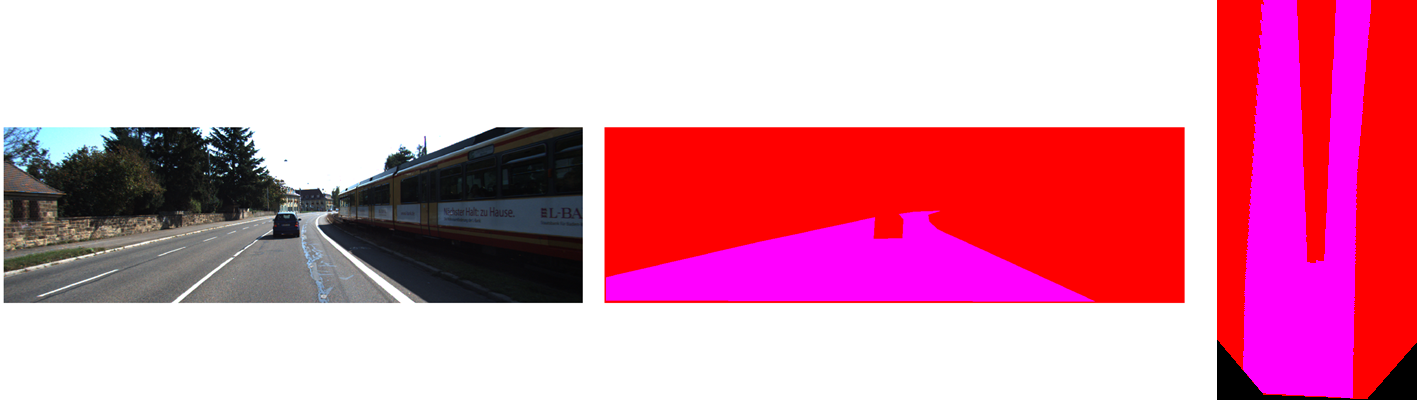
\includegraphics[width=0.75\linewidth]{gt.png}
    \caption{Image, the ground truth and BEV of ground truth from KITTI benchmark. }
    \label{fig:Kitti}
\end{figure*}

LiDAR point clouds in KITTI road benchmark are collected using Velodyne’s high-resolution LiDAR, when operated in the single return mode, returns 1.3 million points per second and will have 64 channels. 
While in real world deployment, we often find LiDARs with 16 or 32 channels. The motivation of this study is to study firstly the impact of pointcloud's spatial resolution on the quality of the road segmentation task, secondly propose geometrical features, as surface point normals that could complement standard features, thirdly augment or fuse these features with appearance features from the Camera (RGB values, and HOG features for windows centered around the camera re-projected point from the pointcloud. We also report the effect of the subsampling the pointcloud in the elevation ($\phi$)

In the current work, we consider the LoDNN (LIDAR-only deep neural network) \cite{lodnn2017} to carry out road detection. The dataset considered are LiDAR point clouds from KITTI road benchmark were used to develop LoDNN and is among top-performing LiDAR only algorithms in the benchmark\cite{Fritsch2013ITSC}.

\subsection{Road segmentation \& Ground Extraction}
Ground extraction and road segmentation are different problems treated in the literature. Ground surface extraction is the problem of removing points on flat surfaces including drivable areas, roads, lanes, footpaths, and open ground. While road segmentation is restricted to extracting the surfaces corresponding explicitly to the road surface. Ground extraction removes a large number of of points for the subsequent obstacle detection tracking and classification steps. Random sampling with consensus (RANSAC) methods , Normal estimation and Hough based methods are among the most popular approaches for this task.

Lidar pointcloud feature extraction has been a key domain, with various heuristics to represent a set of points as a discretised image which can then be used for training a DNN (Deep Neural Network). In this study we shall focus on feature extraction for LiDARs with a spherical coordinate system. Cartesian grids, or BEV images (see figure \ref{fig:pointcloud_features}), which are Occupancy grids over the X-Y axis are evaluated over which elevation (Z-axis) features are calculated such as average height and intensity, standard deviation measures \cite{lodnn2017}. Alternative representations include Front view or Spherical coordinate depth images \cite{wu2018squeezeseg}, \cite{lyu2018chipnet} where authors use images obtained by discretising the elevation and azimuthal angles and using the average distance within each cell.

Chen et al. \cite{chen2017lidar} built a depth image in spherical coordinates, with each pixel indexed by set of fixed azimuth values $\phi$ and horizontal polar angles ($\theta$), with intensity equal to the radial distances ($r$). Authors assume for a given layer (a given $\phi$) all points belonging to the ground surface shall have the same distance from the sensor along the $x$ axis. The $v$-disparity of a given pixel $(p,q)$ is calculated as:

\begin{equation}
\label{eq:LidarHistogram}
\Delta_{p,q} = \frac{1}{x(p,q)}=\frac{1}{d_{p,q}\cos(\phi_{p,q})\cos(\theta_{p,q})}
\end{equation}
%\todo[color=blue!40]{LR: I have checked the article until here, no corrections from this line has been done}

Since all ground points in row $q$ will share a similar $x$ coordinates, they get aggregated into the same bin, and of the histogram assuming the road is laterally flat, the 
high-intensity values in the histogram will draw a line (since the value of 
$\Delta_{p,q}$ will change linearly as we traverse the values of $\varphi$). 
Besides road plane parameter estimation, one can also perform 
online obstacle detection \cite{ravi2018real}.

LoDNN (Lidar Only Deep Neural Networks) \cite{lodnn2017} is a FCN (Fully Convolution Network) based binary segmentation architecture, with encoder containing sub-sampling layers, and decoder with up-sampling layers. The architecture constitutes of a core context module that performs multi-scale feature aggregation using dilated convolutions as shown in figure \ref{fig:lodnn}. ChipNet \cite{lyu2018chipnet} is a DNN-based algorithm
implemented on a FPGA, which is also a FCN based architecture with a encoder, a branched convolutional block, ChipNet block containing filters with ($1 \times 1 \times 64 \times 64$, $3 \times 3 \times 64 \times 64$, $3 \times 3 \times 64 \times 64$) convolutional kernels in parallel.

Camera-Lidar based represesntation learning includes work by authors \cite{lidarcamnet2019} who work on front view images, with upsampled depth maps and RGB images as inputs, while performing early fusion (use an input of $W \times H \times 6$ as input to the LoDNN network), late fusion (Two parallel streams are trained on LIDAR \& RGB images independently until layer 20 in the LoDNN network), and finally cross fusion (usage of trainable scalar weights combining channels across the two streams).

LoDNN the deep learning architecture from \cite{lodnn2017} is an FCN designed for semantic segmentation, has a six-channel input layer, an encoder, a context module and a decoder which returns confidence map for the road. The six-channel input is derived from unstructured point cloud by taking the top view. The number of points; mean reflectivity; mean, standard deviation, minimum, and maximum elevation are calculated and encoded as top view images to get the six-channel input. The output of the model is a confidence map where the probability of whether corresponding points belong to the road is represented in each pixel. Authors use a binary cross-entropy loss. 

\begin{figure*}
    \centering
    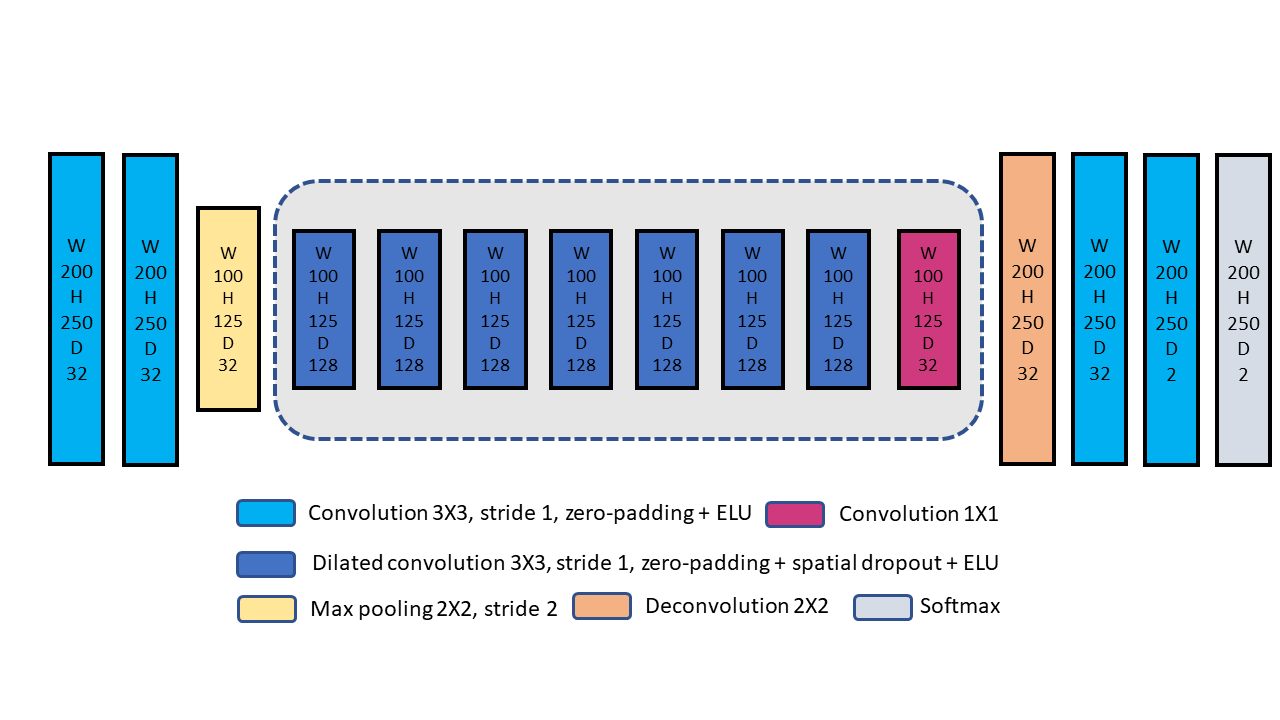
\includegraphics[width=0.85\linewidth]{loDNNArchitecture.png}
    \caption{LoDNN Architecture from \cite{lodnn2017}. }
    \label{fig:lodnn}
\end{figure*}

\subsection{Effect of spatial resolution}
Authors \cite{roynard2018classification} perform Classification of Point Cloud for Road Scene understanding where their pointcloud obtained with multiple lidars were subsampled to maintain a resolution of 2cm. Authors remark while there has been no study on the influence of subsampling on classification quality, maintaining  a scale below the discretization step of the voxel grid, the would keep their results unchanged. Authors \cite{hackel2016fast} devise a multi-scale neighbourhood to learn features that are robust to strong variations in pointcloud density.

In this study we evaluate the effect of subsampling the pointcloud on the performance of DNN models that perform road segmentation. Our key motivation lies in the supposition that information lost by subsampling can effectively be compensated by geometrical features as well as fusion with classical image domains features, in our case HOG (Histogram of Oriented Gradients) \cite{dalal2005histograms}.

\section{Feature Extraction for Representation learning}

The input point cloud is converted into 6 channel input. The points which are between 2 and 27 meter infront, and till 10 meter both sides of the lidar are taken to create the input. We refer to these as classical feature extraction. Thus the grid is 20 meters wide, $y \in [−10, 10]$, and 40 meters long, $x \in  [6, 46]$. This grid is divided into cells of size $0.10 \times 0.10$ meters. The number of points; mean reflectivity; mean, standard deviation, minimum, and maximum elevation are calculated per grid cell and is encoded in an image. Thus our input dimensions will be $400 \times 200 \times 6$. 

\begin{figure*}
    \centering
    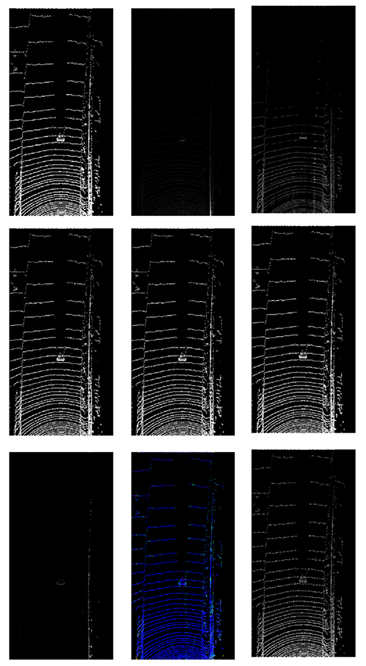
\includegraphics[width=0.465\linewidth]{features__new.png}
    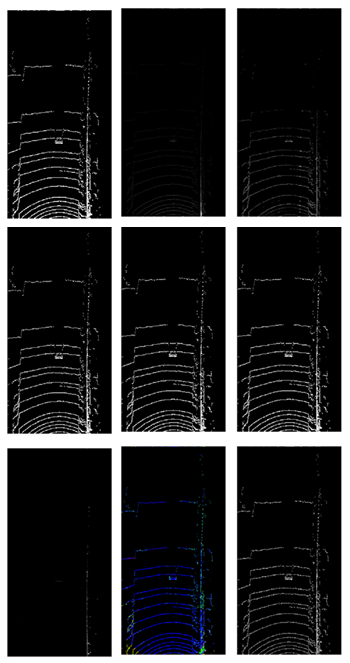
\includegraphics[width=0.45\linewidth]{sub_sample_features__new.png}
    \caption{Left Panel : Features visualized for 64 channel LiDAR.[From top to bottom, left to right] BEV of LiDAR, Number of points per grid, mean reflectance, max elevation, min elevation, mean elevation, standard deviation of elevation, geometrical features, HOG features. Right Panel : Features visualized for sub-sampled point cloud.}
    \label{fig:pointcloud_features}
\end{figure*}


The the confidence map generated is generated by the model. Each pixel value specifies the probability of whether corresponding grid cell of the region belongs to road. The confidence map is thresholded at 0.5 and is used to segment the LiDAR point cloud.

LoDNN network is used to carry out road detection using only LiDAR data. As there is no implementation of LoDNN publicly available, the implementation is done using Python and Keras with TensorFlow. In LoDNN, features such as mean and standard deviation are derived from unstructured point cloud and encoded as top-view images. Then these top-view images are fed into the LoDNN model to get a road confidence map. Instead of Max unpooling layer specified in \cite{lodnn2017}, we use a deconvolution layer. Besides this modification, we have followed the authors implementation of the LoDNN.

\subsection{Geometrical Feature Extraction}
The geometrical feature that we use are surface point normals, and we compute them 
building a depth image in spherical coordiantes as in Chen et al. \cite{chen2017lidar}. Inspired by the work of Nakagawa et al. \cite{nakagawa2015estimating} that estimates surface normals using depth image gradients, we estimate points normals using spherical image gradients.
In fact, a given pixel $p = (i,j)$ in the spherical image corresponds a $3$D point $P$ using the inverse transformation. Let $p_i$ and $p_j$ respectively the horizontal and the vertical neighbouring pixels, they have two corresponding points $P_i$ and $P_j$ in the $3$D space, as well. Since $P$, $P_i$ and $P_j$ compose a local $3$D plane, we can estimate the normal vector of $P$ approximating the two tangent vectors at the local surface that go from $P$ to $P_i$ and from $P$ to $P_j$. In other words, we use pixels $p$, $p_i$ and $p_j$ to estimate directional derivatives $v_i$ and $v_j$  at $P$ as tangent vectors of the surface at $P$. Finally the normal vector is obtained as the cross product of the two tangent vectors $ n = v_i \times v_j$. 
Once estimated the surface point normals in the spherical image we project them back to the point cloud and generate BEV images containing geometrical information. This add $3$ supplementary channels to the input images.  

\subsection{Fusion with HOG features in Camera domain}
Using the calibration information we re-projected input points from the point-cloud domain to the image grid. Basically, we map each point $P$ in the input point cloud to a pixel $p$ in the camera domain. For the moment we  assume that each point is in the FOV of the camera. Using this association we evaluate HoG feature vector for each mapped point in the images. Once all the HoG feature vectors are computed, we aggregate them together and we project them to the first $6$ principal components using PCA, in order to reduce the number of features. The choice of the number of components is purely empirical. In this way for each point in the point cloud we have a $6$ dimensional feature vector associated and we can projected it to the BEV images.

\section{Results}
KITTI road segmentation dataset \cite{Fritsch2013ITSC} is used for this experiment. Since the test dataset's ground truth is not publicly available, 289 training samples from dataset is split into training, validation and test sets for the experiments. Validation and test sets has 30 samples each from three categories of KITTI benchmark and the remaining 229 samples are taken as training set.

\textbf{Subsampling method} :
Since we do not have 32-Channel LiDAR based point cloud, we subsample pointclouds in the KITTI dataset. Our idea is to associate at each point the layer that acquired it, and keep only points acquired by one every two layers. To do so, we compute the azimuthal coordinates of the points and split them in $64$ bins, each one corresponding to a layer. 

\noindent  These results were evaluated  on Intel i7, Titan XP GPU machine. Adam optimiser with initial learning rate of 0.0001 is used to train LoDNN model on this dataset. The model was trained for 125 epochs with a validation split of 10\%. Loss function used for training is Jaccard. The F1 score\cite{Fritsch2013ITSC} was used to evaluate the accuracy of the DNNs. The precision and recall were calculated for the entire test set along with the F1-score was calculated.

\begin{figure}
    \centering
    \includegraphics[width=\linewidth]{ROC.eps}
    \caption{Precision-Recall Curve for various features with and without sub-sampling.}
    \label{fig:roc}
\end{figure}
    
\begin{table}
\centering
\begin{tabular}{|l|c|c|c|c|} % <-- Alignments: 1st column left, 2nd middle and 3rd right, with vertical lines in between
  \hline
  \textbf{Features} & \textbf{IoU} & \textbf{OA} & \textbf{F1 Score} & \textbf{Time (s)}\\
  \hline
  C             &  0.762 &  0.88 & 0.82 & 0.42 \\
  C + G         & 0.715 & 0.85 & 0.77 & 0.37 \\
  C + H         & 0.71 & 0.84 & 0.76 & 0.38 \\
  C + G + H     & 0.73 & 0.86 & 0.79 & 0.36 \\
  C + S         & 0.77 & 0.88 & 0.82 & 0.39 \\
  C + S + G     & 0.70 & 0.84 & 0.76 & 0.40 \\
  C + S + H     & 0.77 & 0.88 & 0.82 & 0.38\\
  C + S + G + H & 0.74 & 0.86 & 0.8 & 0.58 \\
  \hline
\end{tabular}
\caption{Results obtained on our test set using different sets of features. C: classical features, G: geometrical features, H: HOG features, S: subsampled set.}\label{tab:results}
\end{table}  
    
\section{Discussion}

Reduction in range of road detection was found when sparse point cloud was used. But the accuracy (F1 score) was comparable with that of the dense point cloud. This is also reflected in the Precision-Recall curves in figure \ref{fig:roc} and table \ref{tab:results}. This experiment showed that existing deep learning solutions which are developed on dense point cloud may be used for processing sparse point cloud with no or slight modifications. Low-resolution LiDAR’s usually used in deployment could now aim to perform road segmentation online for various path planning and driving policy tasks. In future work we aim to evaluate  which elevation angles (thus layers) would be provide the highest improve in performance for the road segmentation task.

\section*{Acknowledgements}

We thank authors of LoDNN for their insights and support.

{\small
\bibliographystyle{ieee}
\bibliography{sample}
}

\begin{figure}[!th]
  \centering
  \begin{subfigure}[b]{\columnwidth}
    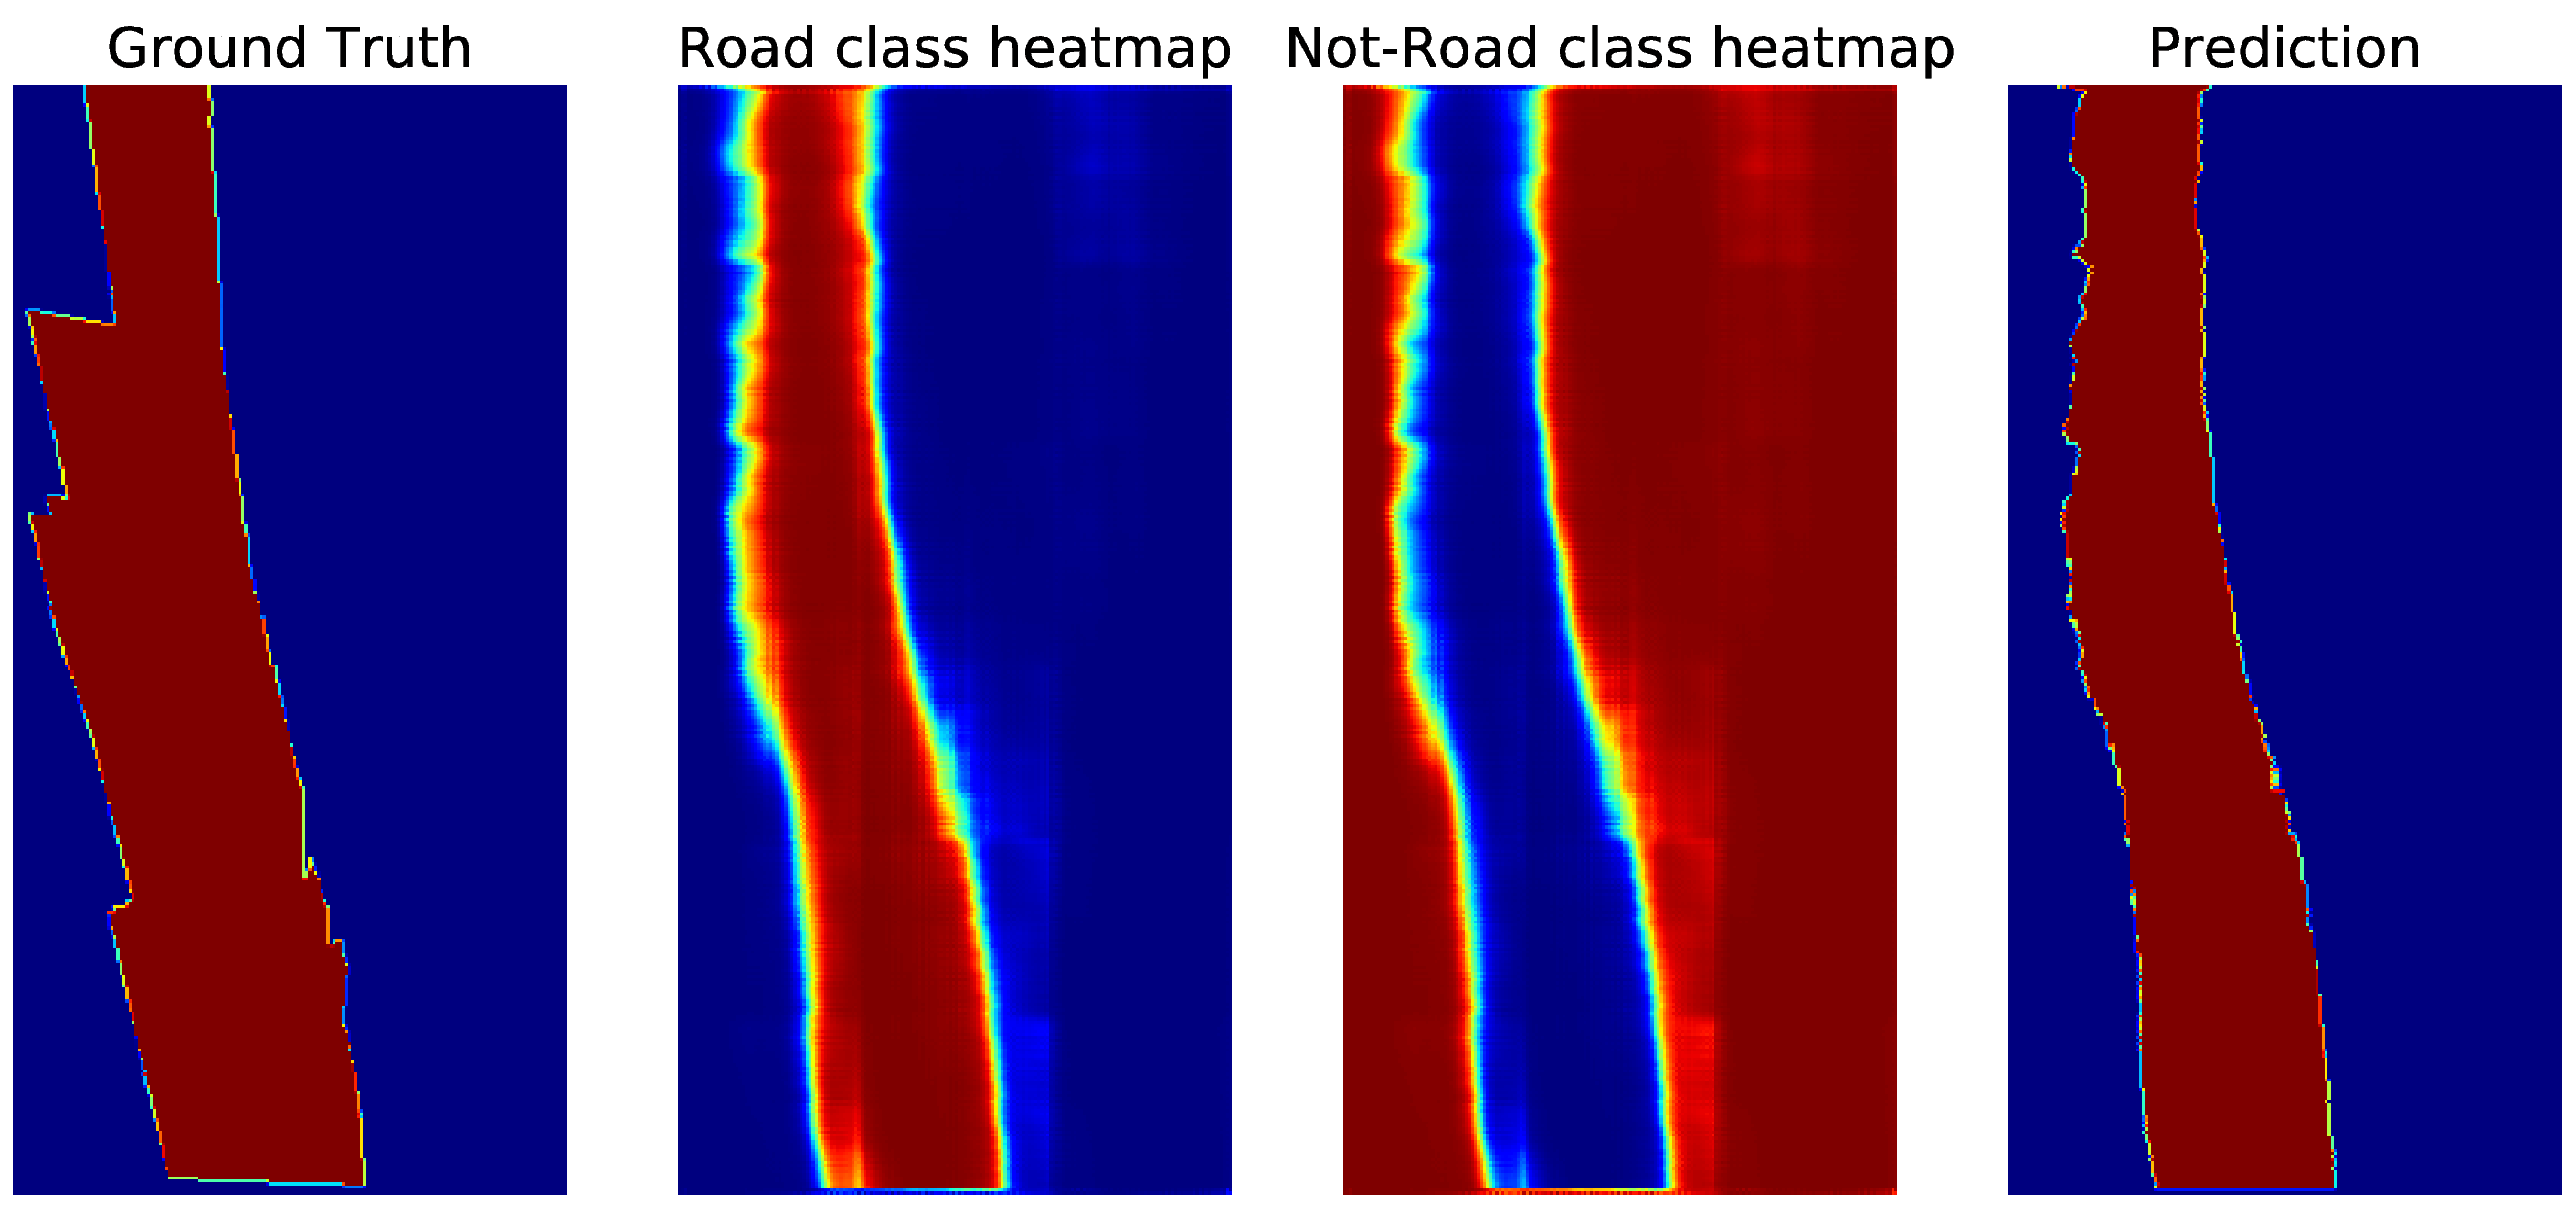
\includegraphics[width=\columnwidth]{pred_classic.png}
    \caption{Classic features}
  \end{subfigure}
  
  \begin{subfigure}[b]{\columnwidth}
    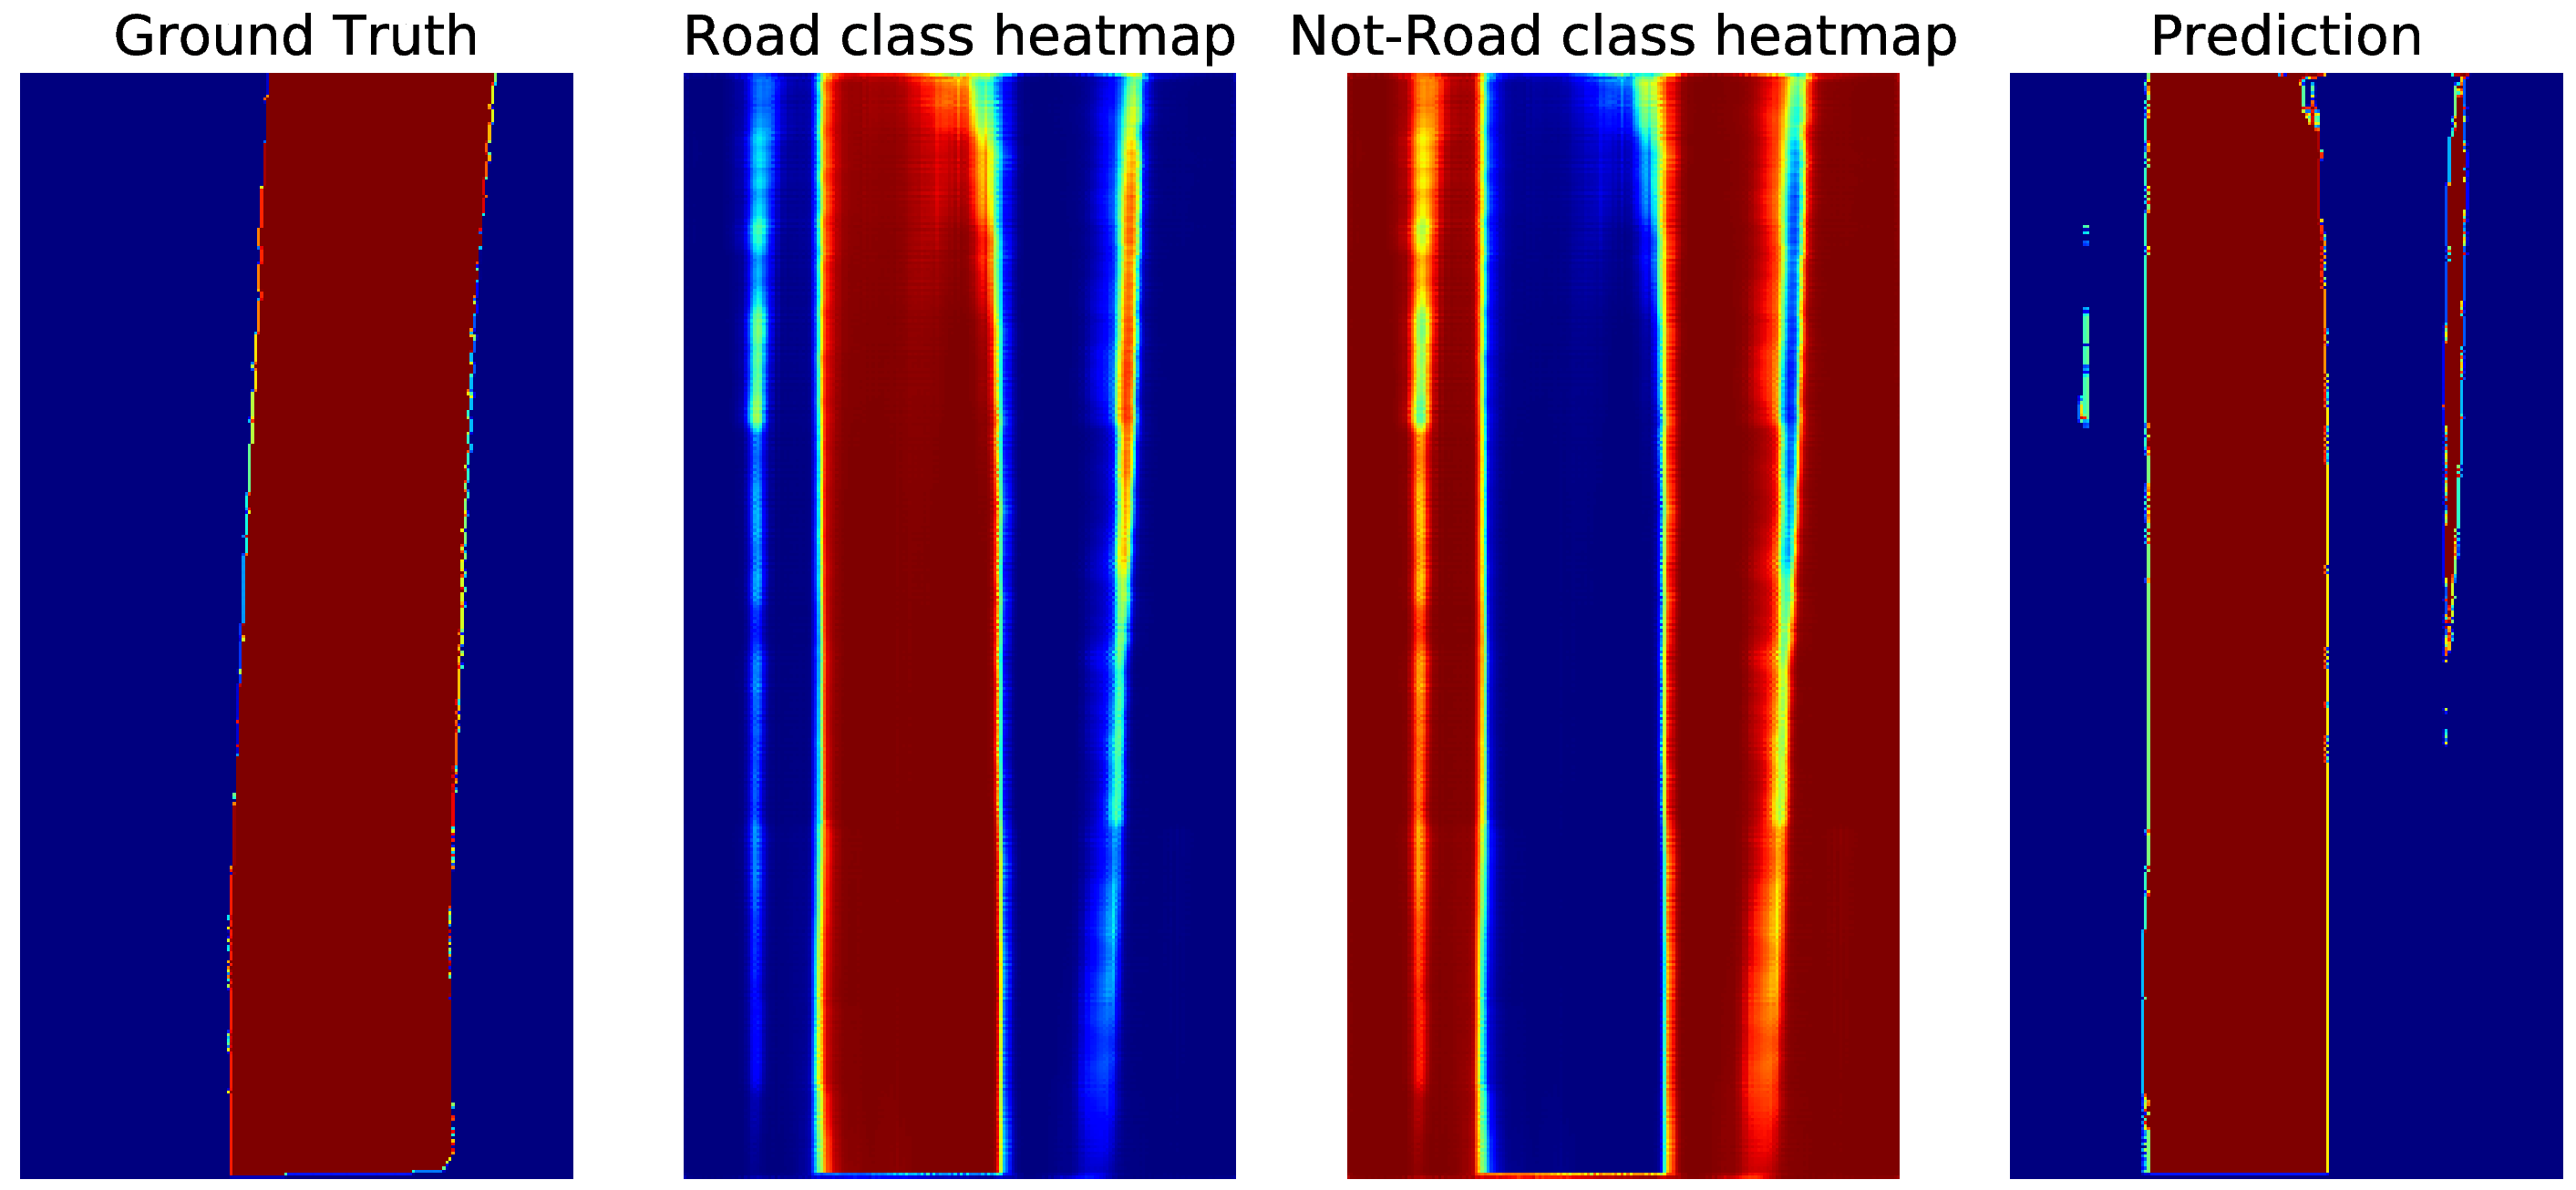
\includegraphics[width=\columnwidth]{pred_classic_geom.png}
    \caption{Classic + Geometric features}
  \end{subfigure}
  
  \begin{subfigure}[b]{\columnwidth}
    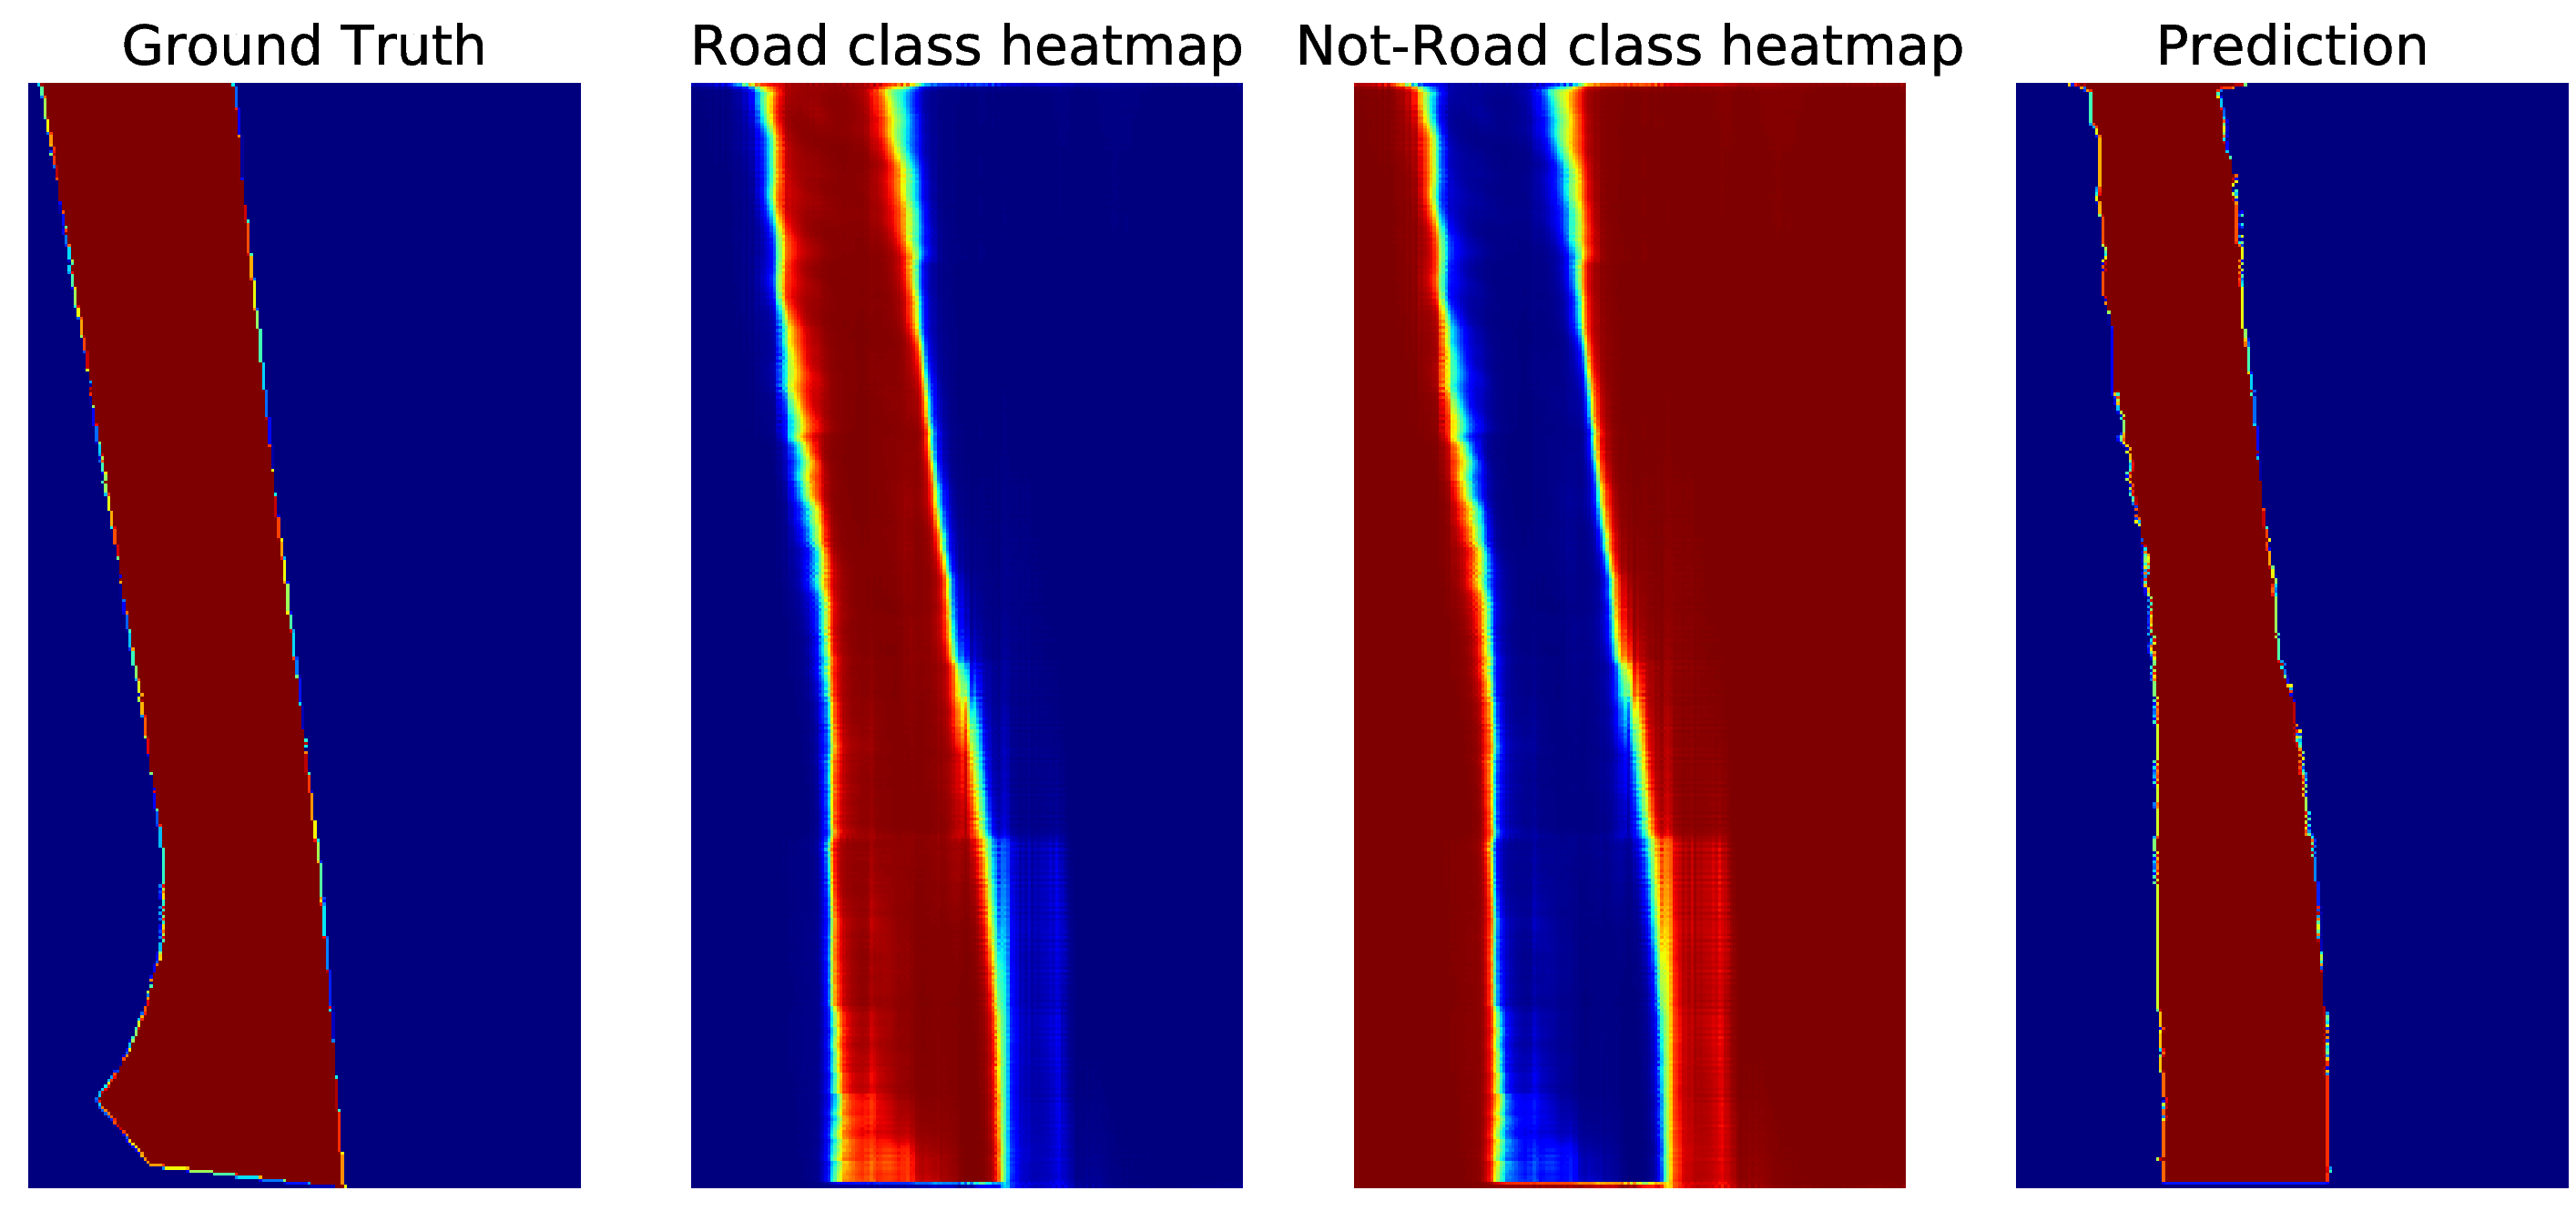
\includegraphics[width=\columnwidth]{pred_classic_hog.png}
    \caption{Classic + Geometric + HoG features}
  \end{subfigure}
  
  \begin{subfigure}[b]{\columnwidth}
    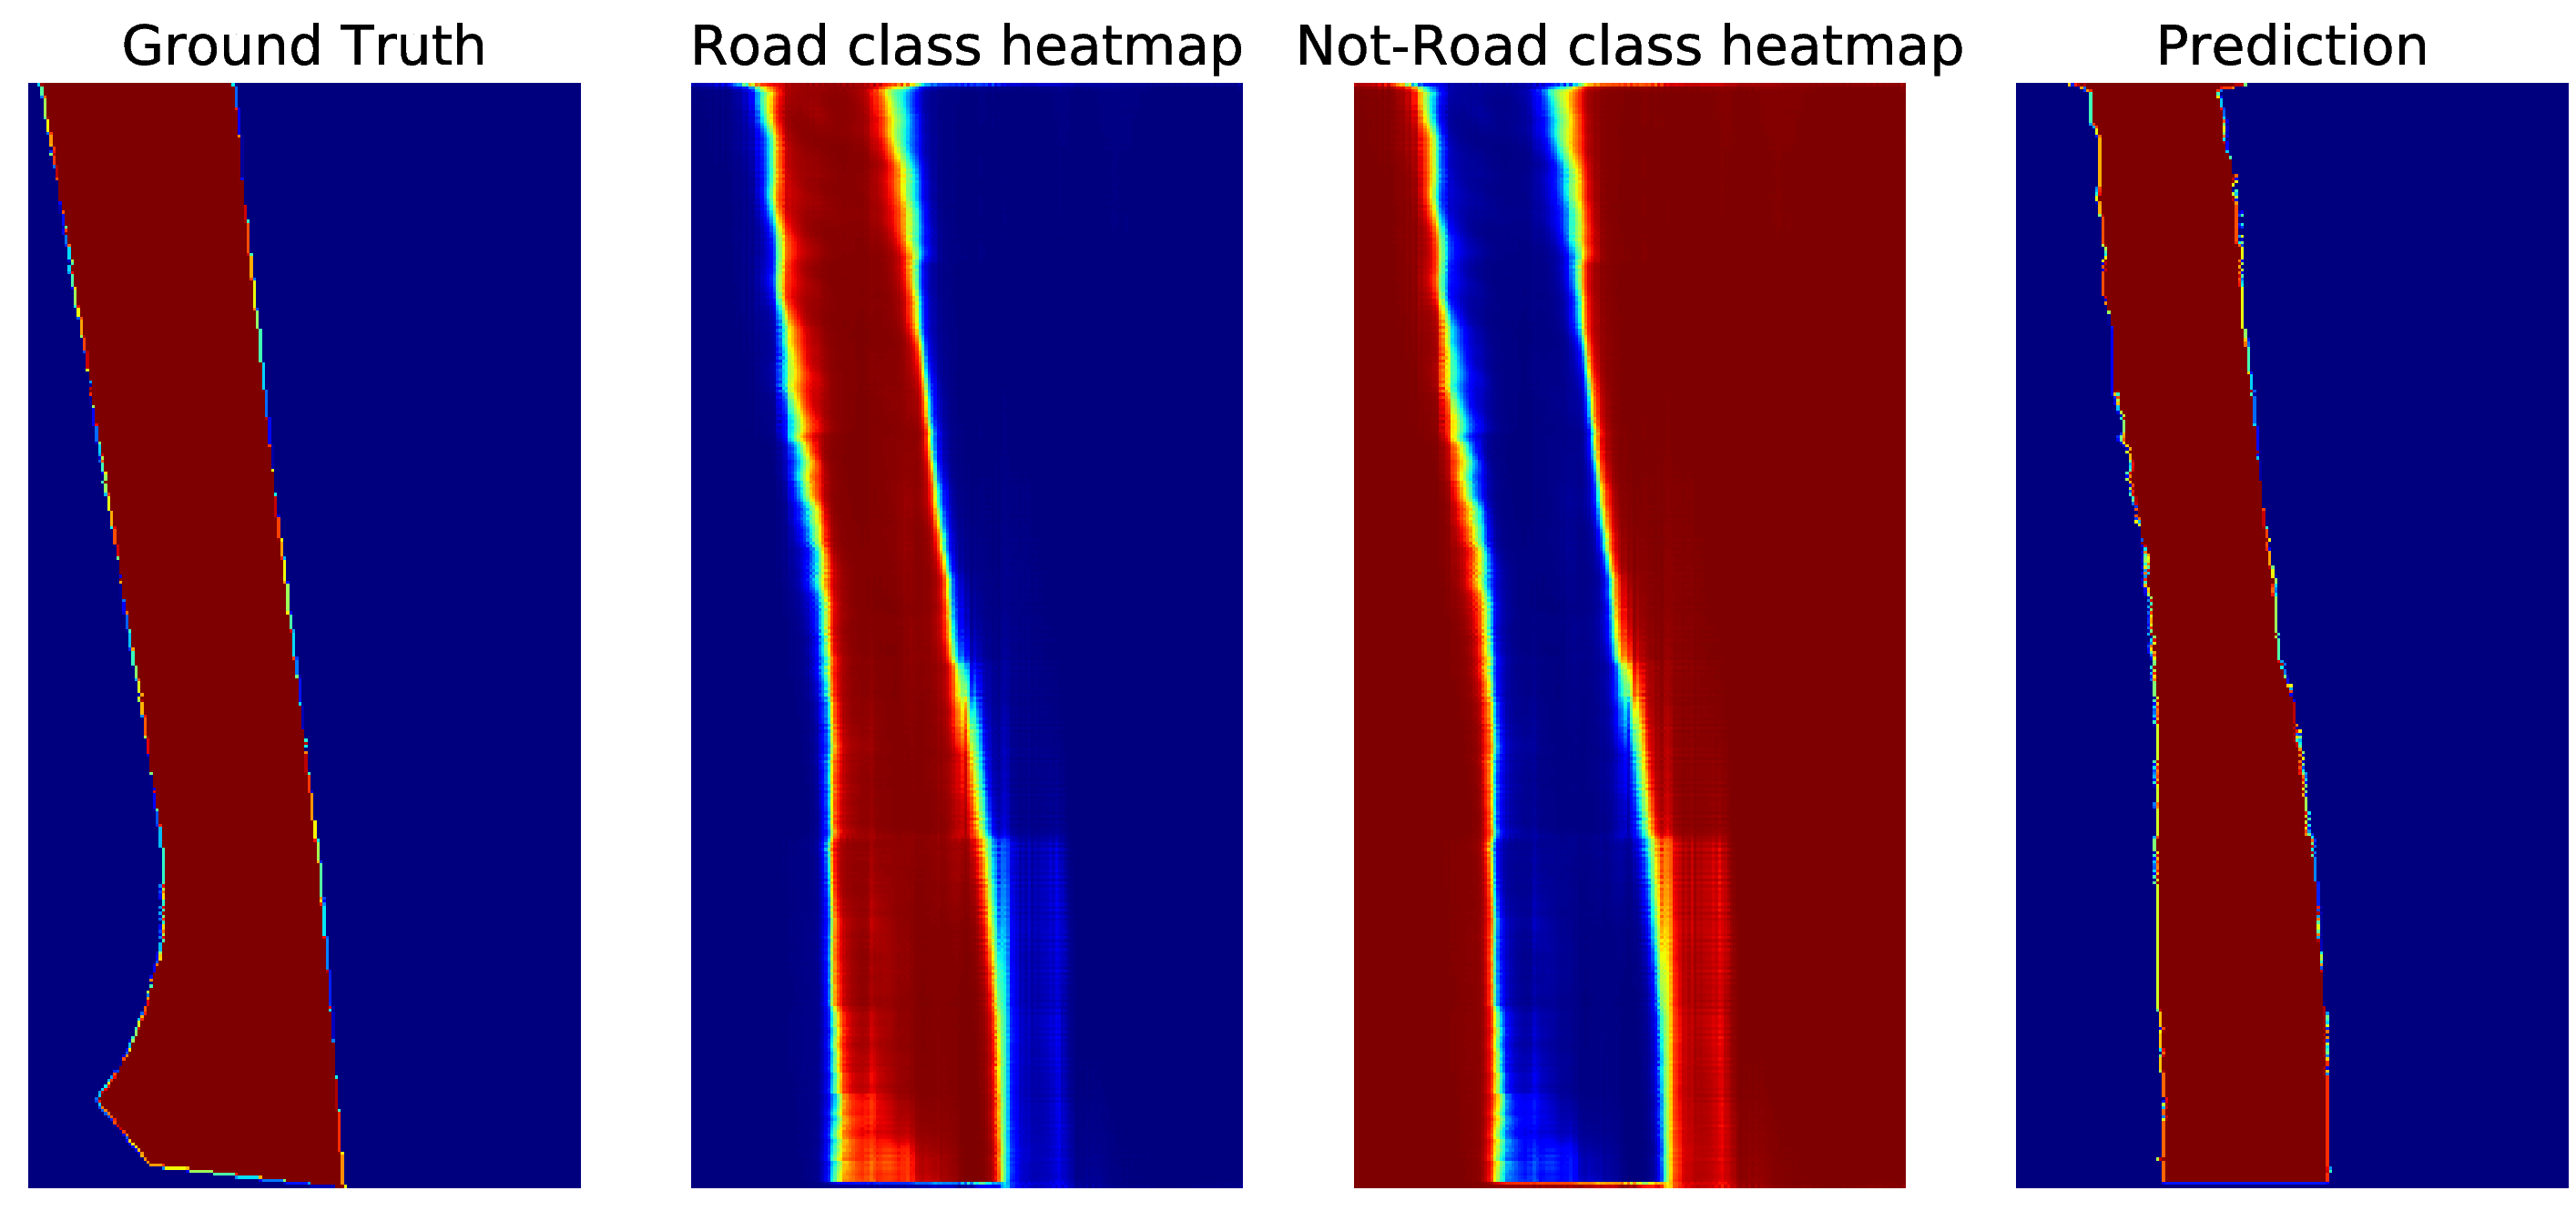
\includegraphics[width=\columnwidth]{pred_classic_hog.png}
    \caption{Classic + HoG features}
  \end{subfigure}
 \caption{Predictions obtained using LoDNN on point clouds with different sets of features.}
 \label{fig:results}
 \end{figure}

 \begin{figure}[!th]
  \centering
  \begin{subfigure}[b]{\columnwidth}
    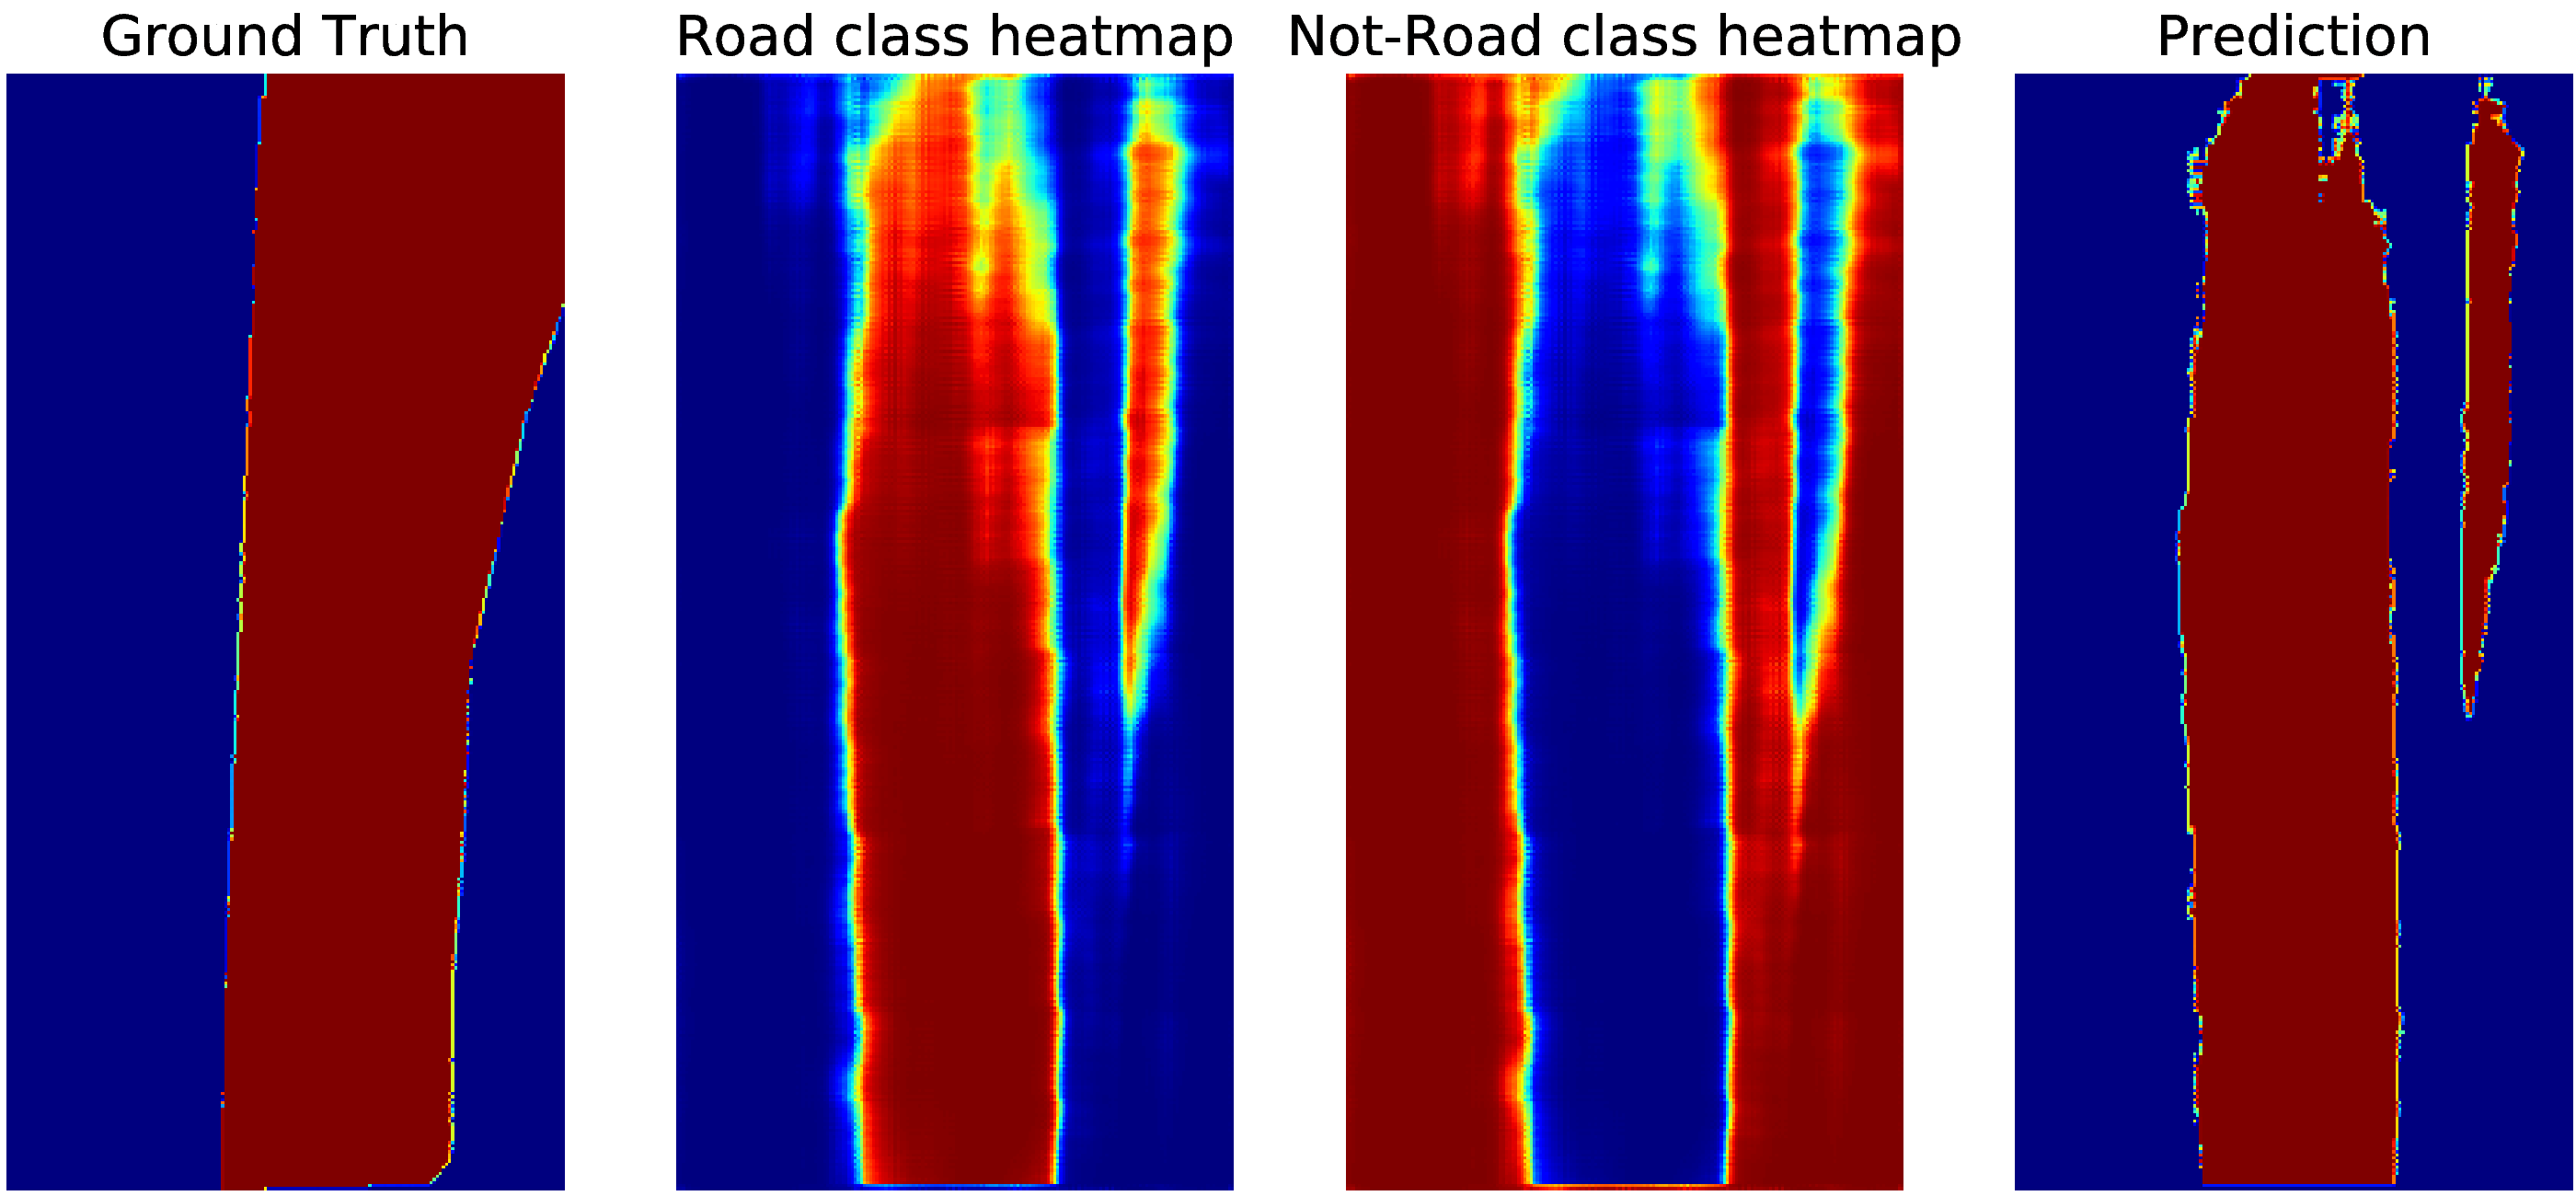
\includegraphics[width=\columnwidth]{pred_classic_sub.png}
    \caption{Subsampled Point Cloud + Classic features}
  \end{subfigure}
  
  \begin{subfigure}[b]{\columnwidth}
    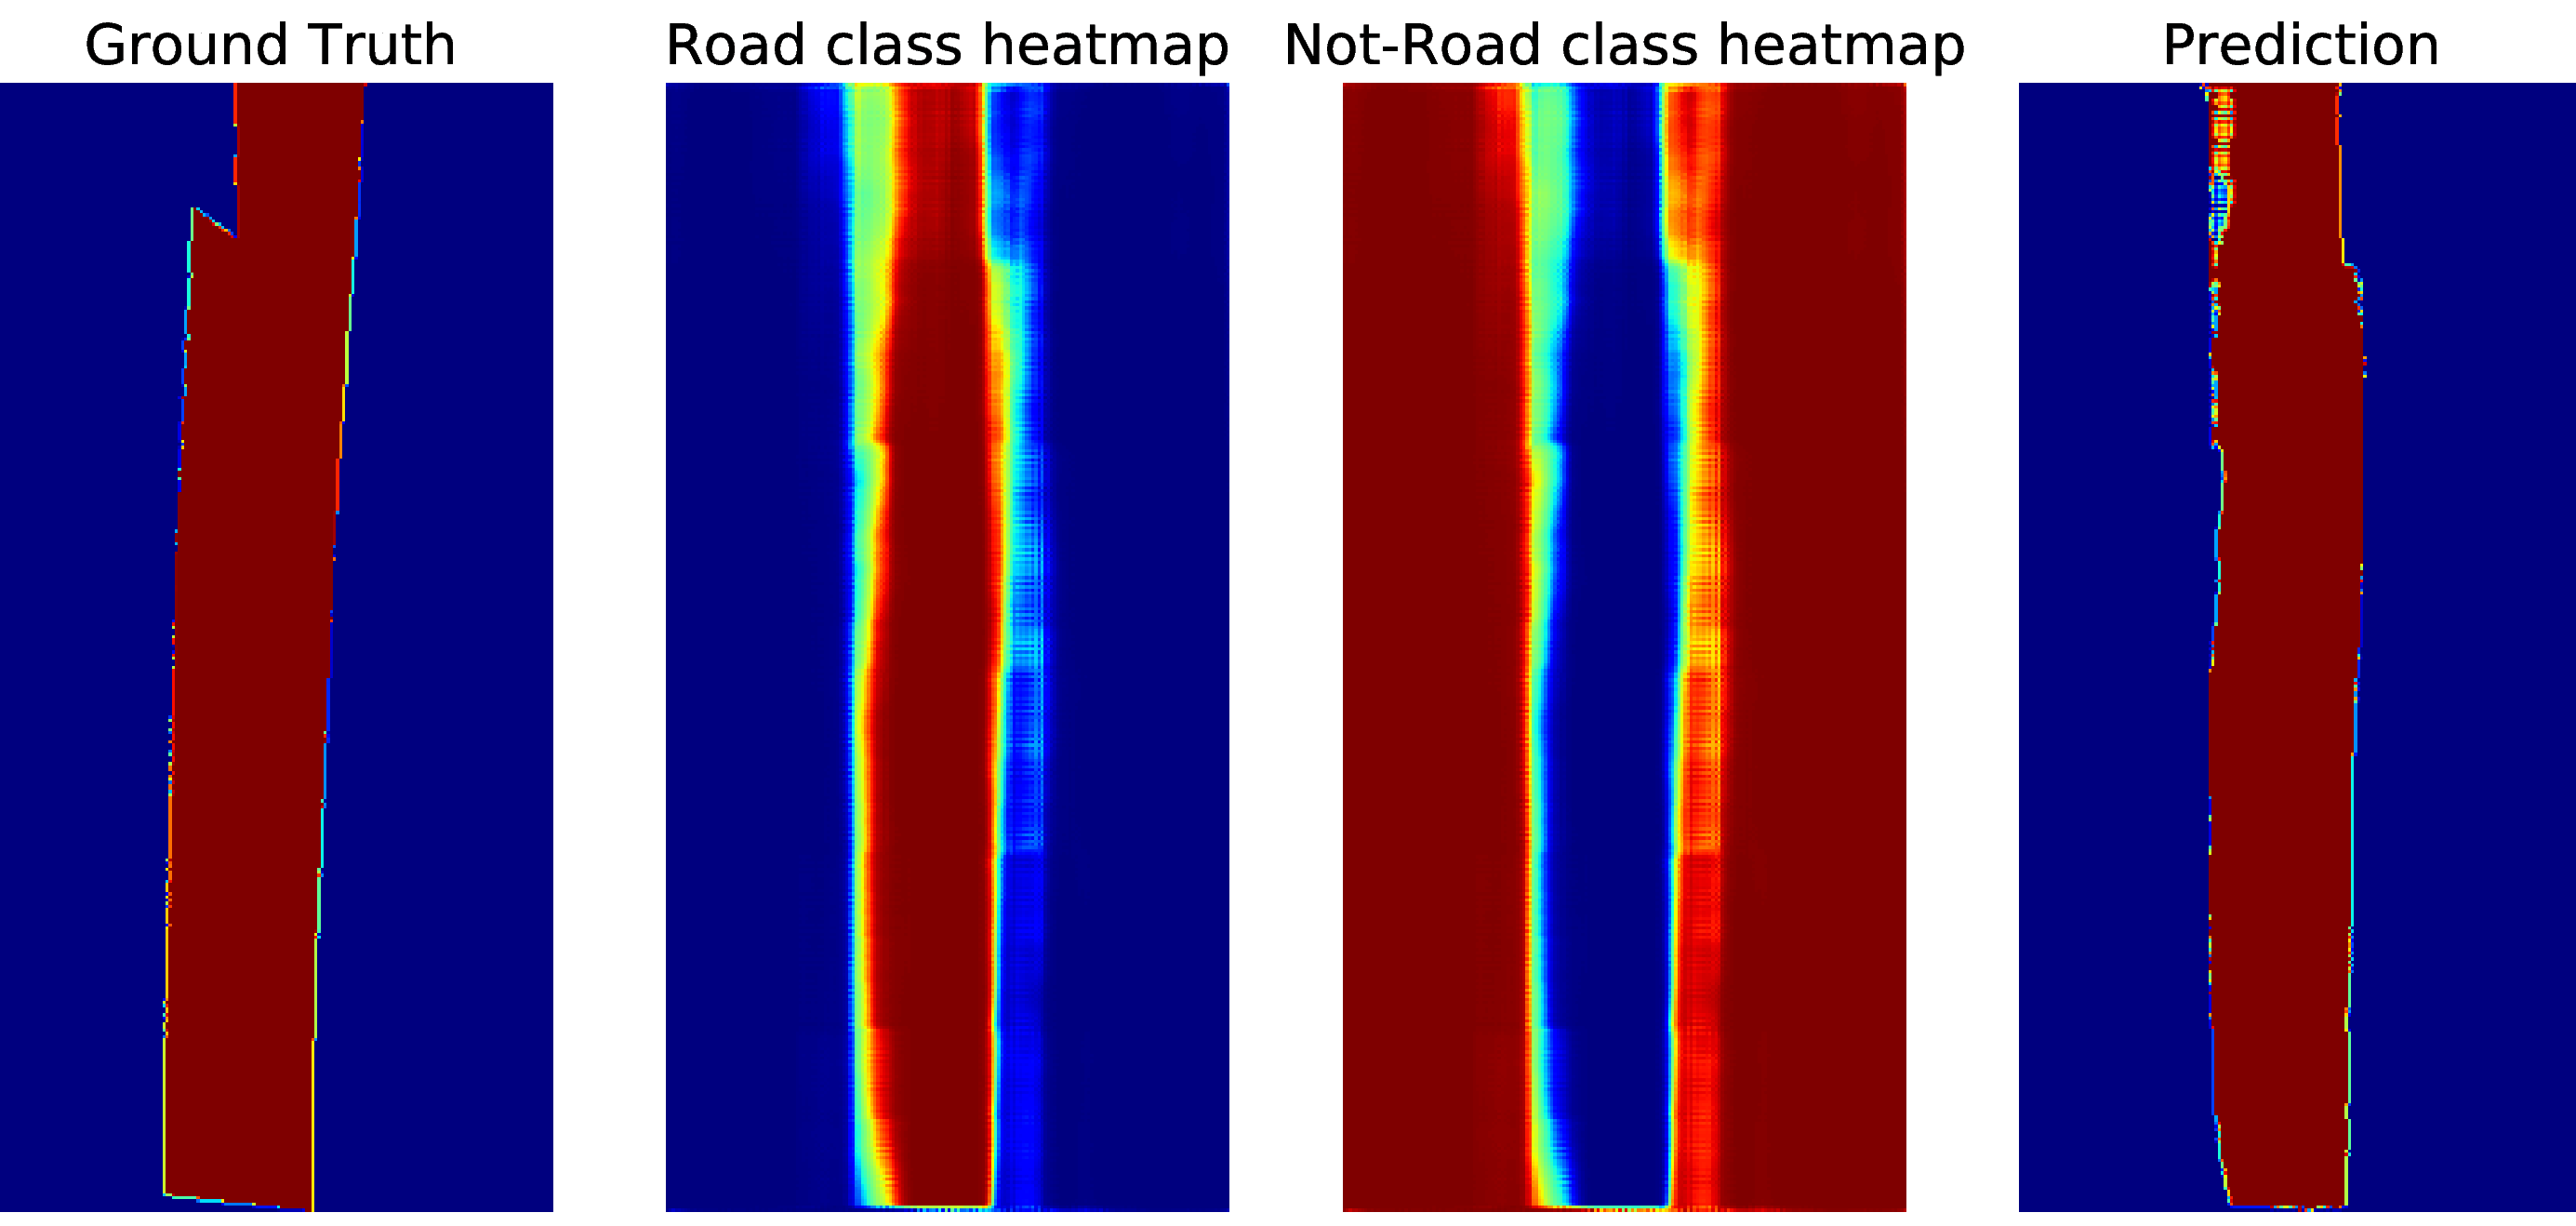
\includegraphics[width=\columnwidth]{pred_classic_geom_sub.png}
    \caption{Subsampled Point Cloud + Classic + Geometric features}
  \end{subfigure}
  
  \begin{subfigure}[b]{\columnwidth}
    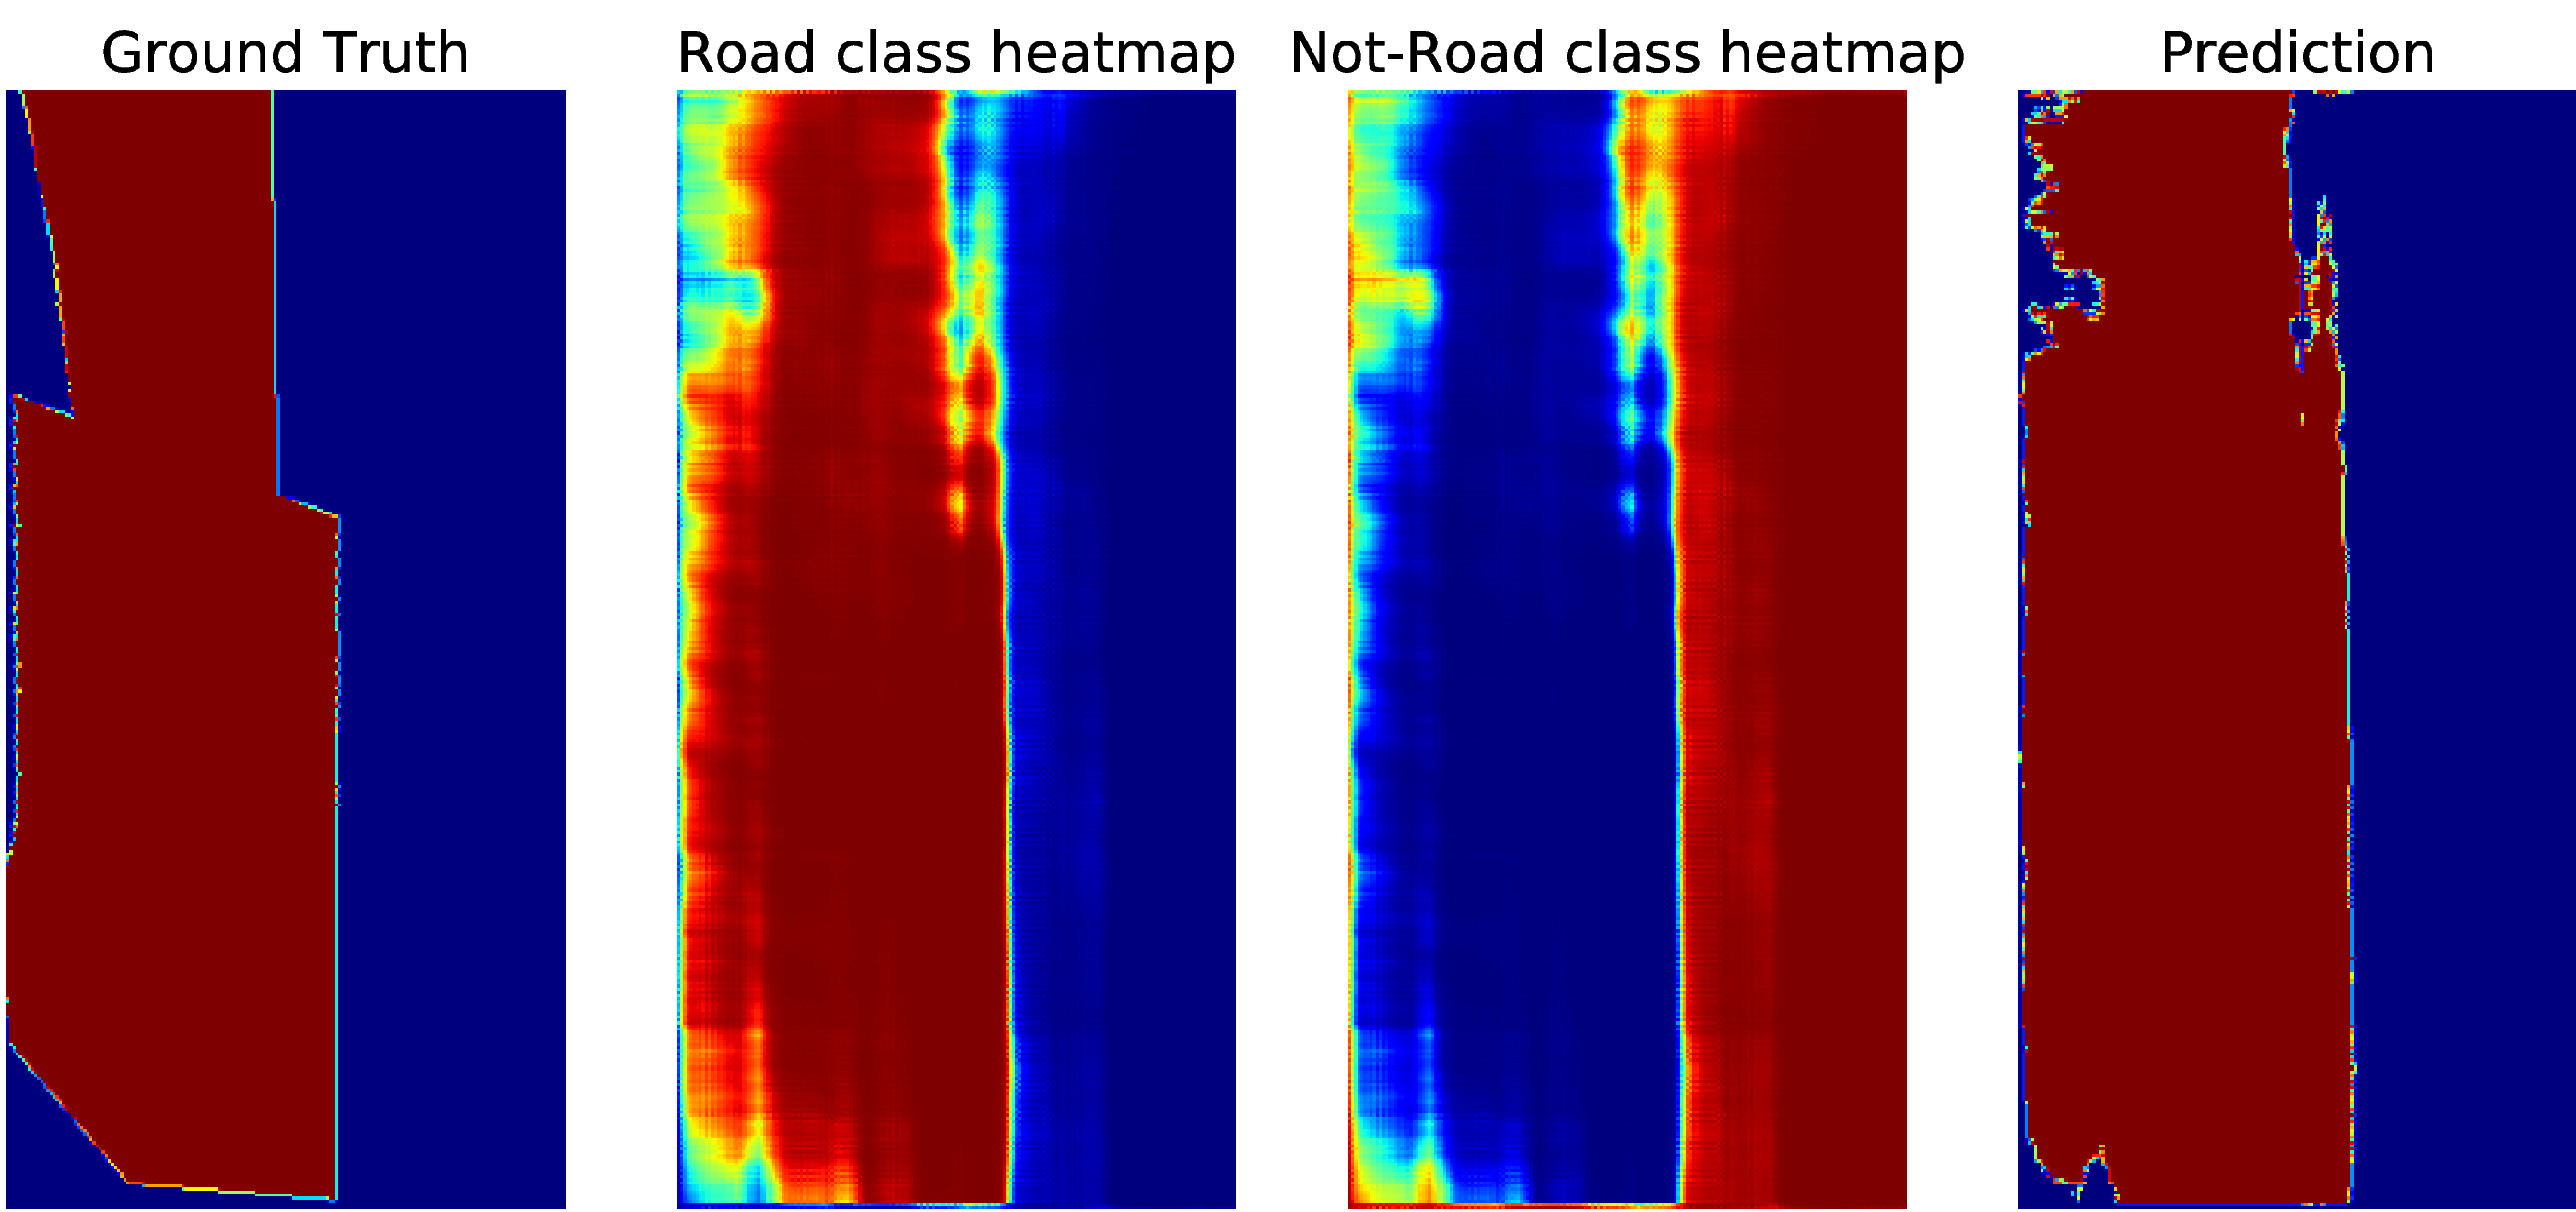
\includegraphics[width=\columnwidth]{pred_classic_sub_hog.png}
    \caption{Subsampled Point Cloud + Classic + HoG features}
  \end{subfigure}
  
  \begin{subfigure}[b]{\columnwidth}
    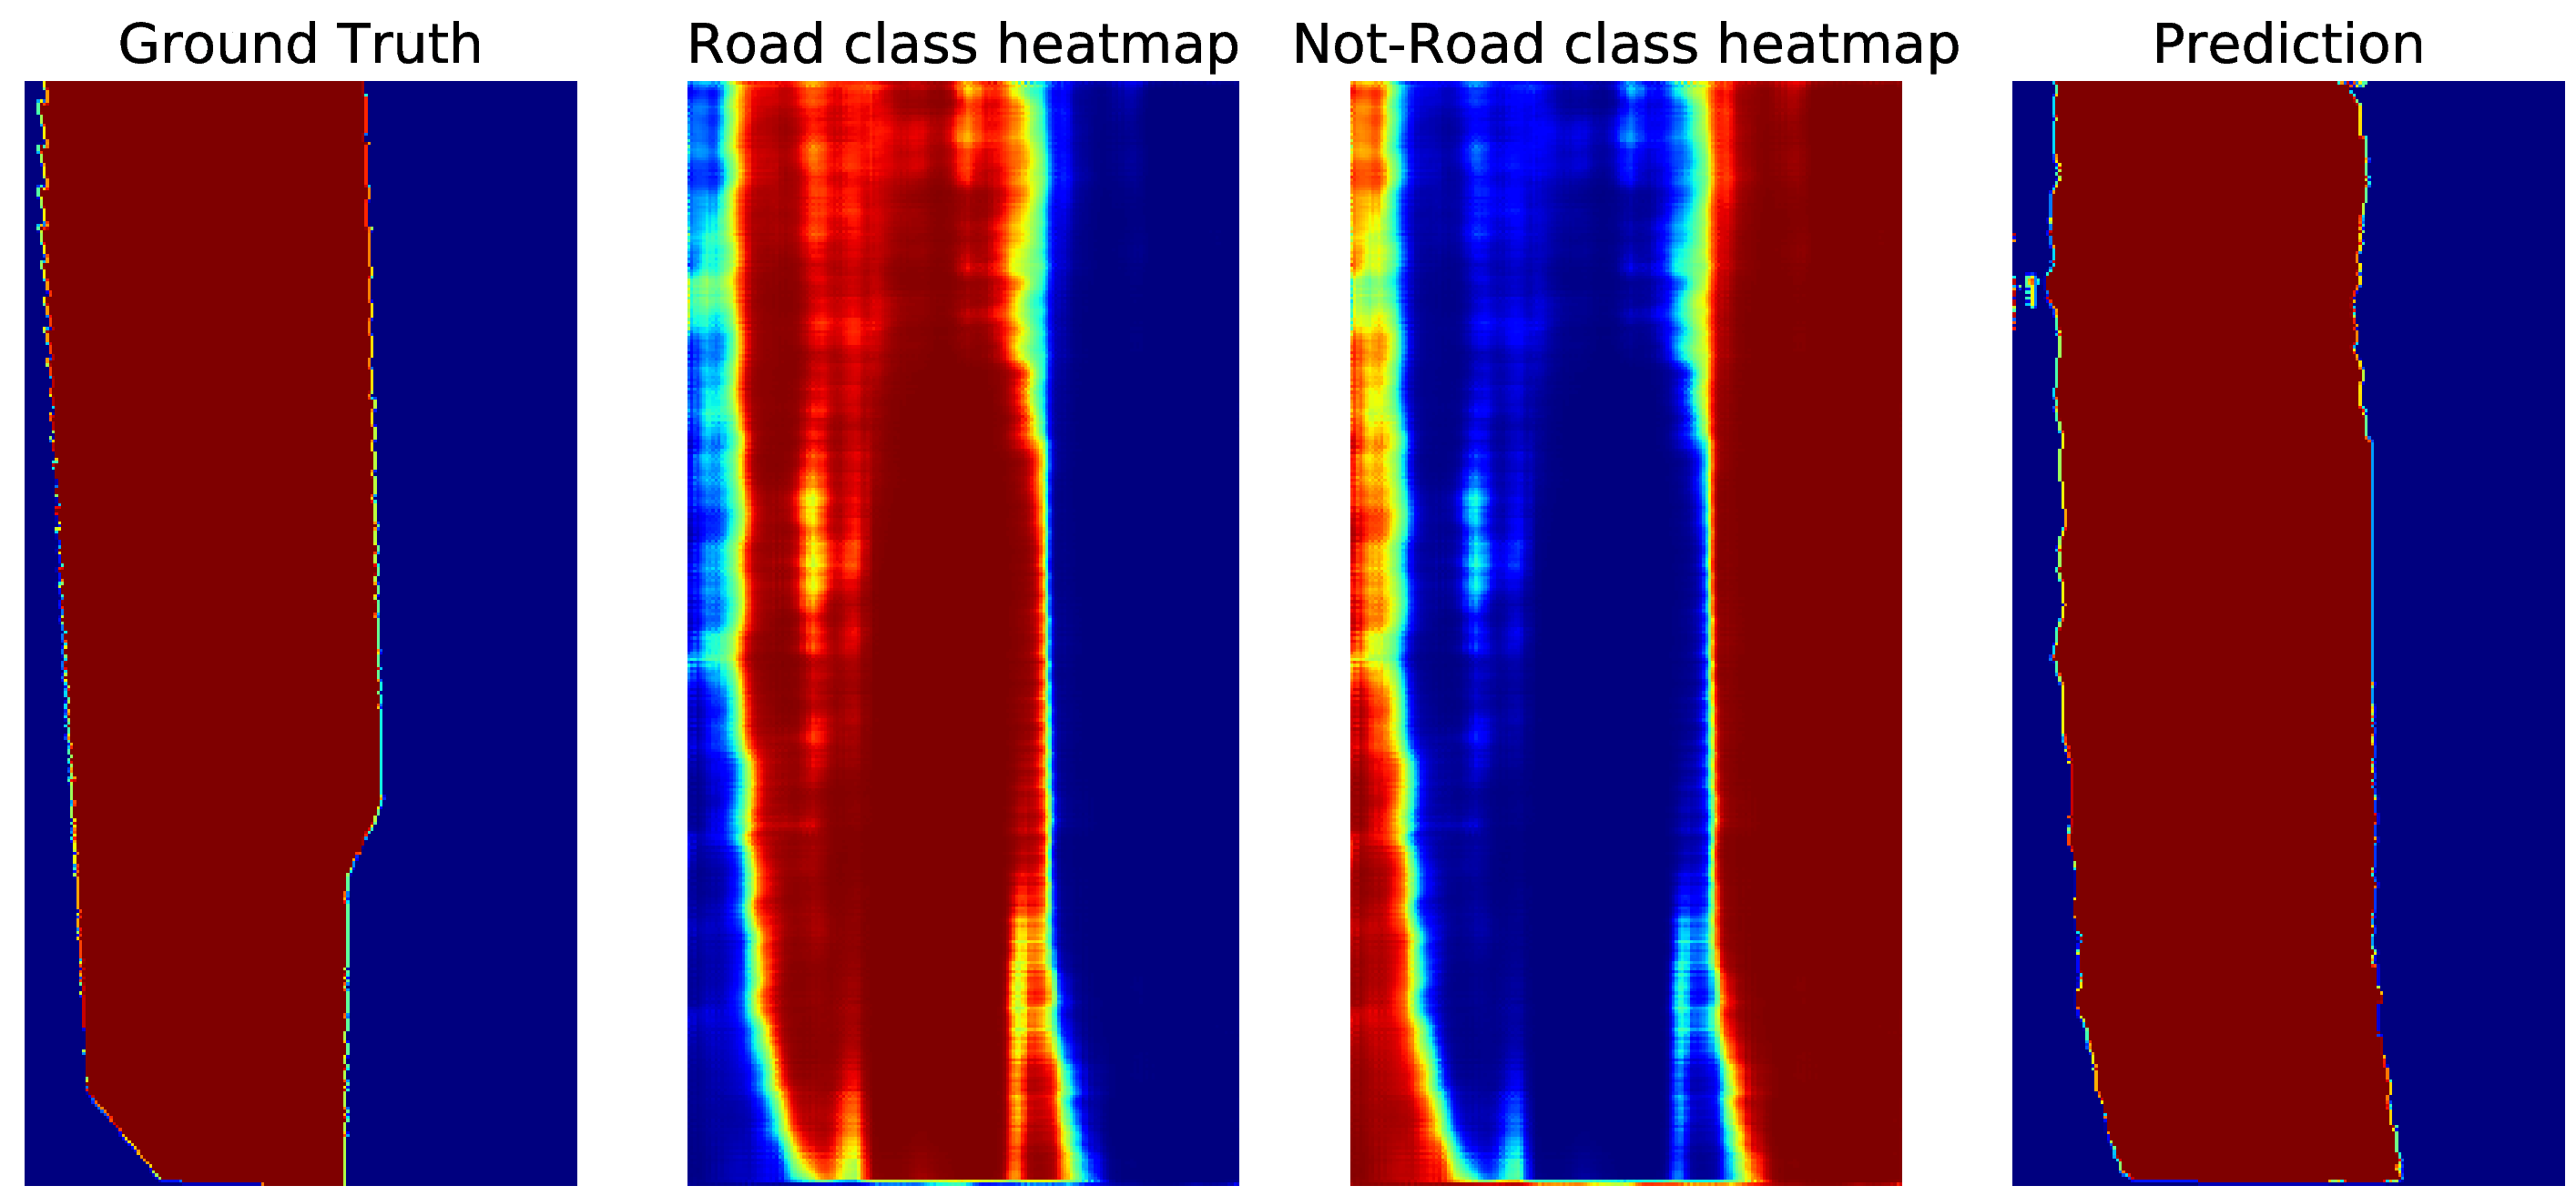
\includegraphics[width=\columnwidth]{pred_classic_geom_sub_hog.png}
    \caption{Subsampled Point Cloud + Classic + Geometric + HoG features}
  \end{subfigure}
 
  \caption{Predictions obtained using LoDNN on subsampled point clouds with different sets of features.}
  \label{fig:sub_results}
\end{figure}

\end{document}